\documentclass{ximera}

\title{Exercises: Shell Method}
\author{Pat Smith}

\begin{document}
\begin{abstract}
Exercises for using the shell method.
\end{abstract}
\maketitle

\begin{exercise}
The region defined by the inequalities $\sqrt{1-x^2} \leq y \leq 1$ for $0 \leq y \leq 1$ is revolved around the $y$-axis. Compute the volume of the resulting solid using the shell method.
\begin{center}
\begin{image}
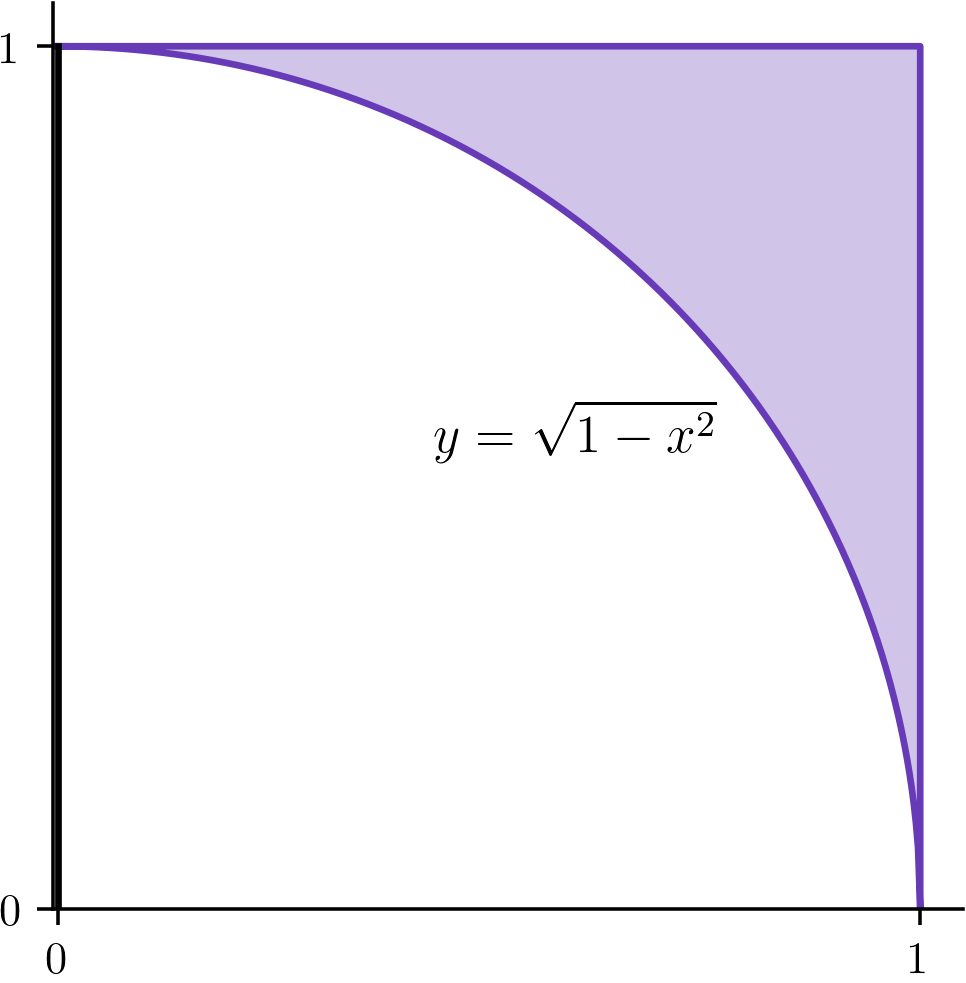
\includegraphics{shell/shell03.png}
\end{image}
\end{center}
\begin{itemize}
\item When the slicing variable is $x$, the radius of a shell is the \wordChoice{\choice[correct]{horizontal}\choice{vertical}} distance from an $x$-slice to the axis of rotation. Thus
\[ r(x) = \answer{x} - \answer{0}. \]
\item The height of an $x$-slice is equal to
\[ h(x) = \answer{1 - \sqrt{1 - x^2}}. \]
\item The volume is equal to the integral of $2 \pi r h$, so 
\[ V = \int_{\answer{0}}^{\answer{1}} \answer{2 \pi x ( 1 - \sqrt{1-x^2}) } dx = \answer{\frac{\pi}{3}}. \]
(Note: to compute the integral, split it into two parts and make the substitution $u = 1-x^2$ for one of them.)
\end{itemize}
\end{exercise}

\begin{exercise}
The region in the plane bounded above by the graph $y = \sqrt{1+x^2}$, below by $y = -1 + x + \sqrt{1+x^2}$, and on the left by $x = 0$ is revolved around the axis $x = 1$. Compute the volume of the resulting solid using the shell method.
\begin{center}
\begin{image}
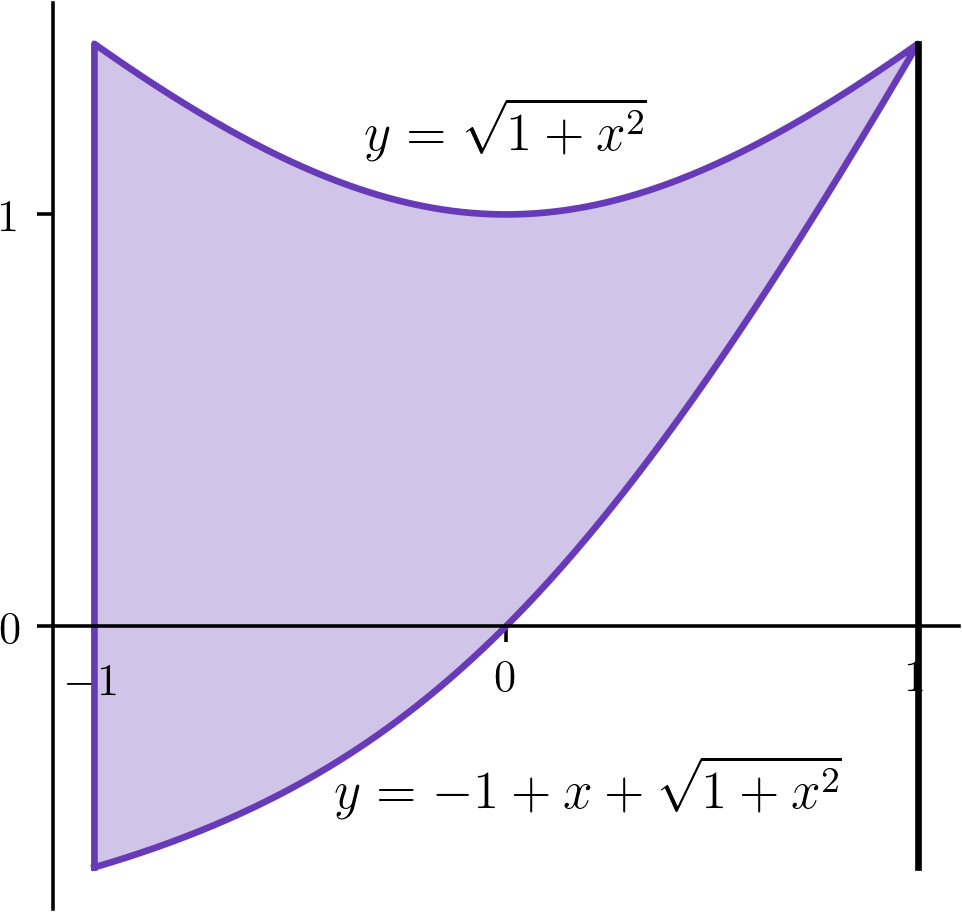
\includegraphics{shell/shell04.png}
\end{image}
\end{center}
\begin{itemize}
\item When the slicing variable is $x$, the radius of a shell is the \wordChoice{\choice[correct]{horizontal}\choice{vertical}} distance from an $x$-slice to the axis $x = 0$. Thus
\[ r(x) = \answer{1} - \answer{x}. \]
\item The height of an $x$-slice is equal to
\[ h(x) = \answer{-1+x}. \]
\item The volume is equal to the integral of $2 \pi r h$, so 
\[ V = \int_{\answer{-1}}^{\answer{1}} \answer{2 \pi (1-x)^2 } dx = \answer{\frac{16\pi}{3}}. \]
\end{itemize}
\end{exercise}





\end{document}
